\newacronym{ctan}{CTAN}{Comprehensive TeX Archive Network}
\newacronym{faq}{FAQ}{Frequently Asked Questions}
\newacronym{pdf}{PDF}{Portable Document Format}
\newacronym{svn}{SVN}{Subversion}
\newacronym{wysiwyg}{WYSIWYG}{What You See Is What You Get}

\newglossaryentry{texteditor}
{
	name={editor},
	description={A text editor is a type of program used for editing plain text files.}
}

\chapter{Overview}

\section{Introduction}

Biochemistry lies at the root of complex biological systems that describe the machinery of life.
In order to understand how we work, we must first understand the complete cascade of events starting from the atomic level.
Because biological systems span several scales of space and time as well as scientific fields, such as biology, chemistry, mathematics, or medicine, it is crucial to communicate advances in biochemistry efficiently between experts with different scientific backgrounds.
Moreover, there is also a growing interest from the general audience to understand how living organisms work.

\begin{figure}
\centering
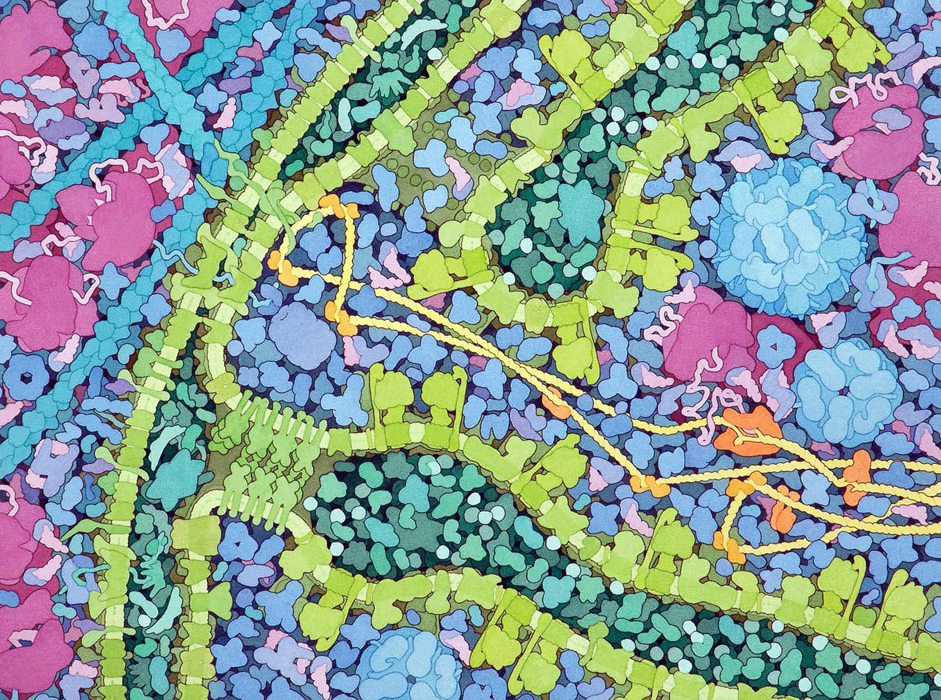
\includegraphics[width=0.95\linewidth]{graphics/Picture12}
\caption{}
\label{fig:david-s}
\end{figure}


Visual communication is undeniably efficient for educating a non-expert audience about the how physiological processes function.
A quick glance into physiological textbooks is enough to realize that they would be close to useless without any illustrations.
Illustrations, such as the ones made by David Goodsell, are often used to convey information in such textbooks.
The illustrator likes to depict entire sceneries on the mesoscale levels, as shown in Figure~\ref{fig:david-s}, which would be impossible to observe otherwise in such detail using current microscopy instruments.
His paintings rightfully balance scientific accuracy and clarity, which makes them very popular because they are accessible to a large audience.
 
The realization of such illustrations, however, is very laborious and also demands highly skilled individuals.
The first step of the creation process consists of gathering knowledge from the scientific literature, in order to thoroughly understand the process that is to be depicted.
This task demands a thorough knowledge of biology, as scientific articles are intended to be read by experts and peers.
Based on gathered information, the illustrator will decide how to compose the scene, i.e., which macromolecular structures should be present, where should they be located, in which quantities, and what behaviour should they exhibit.

The second step of the creation process is the drawing. 
It is important not to confuse the work of a scientific illustrator with the work of an artist.
Although they both aim at conveying a message or an idea, the artist has the freedom to hide his message behind a curtain of abstraction.
On the contrary, an illustrator has to convey a message as clearly as possible in order to expose scientific concepts to an uninformed audience.
This concretely means that the illustrator is bound to a set of logical guidelines in terms of composition, lighting, color-coding or storytelling.

While some illustrators prefer working with paper and pencil or 2D composition software such as Photoshop, the new generation of illustrators grew with 3D rendering and animation packages such as Maya, Cinema4D or Blender, made mainstream by the popularization of digital effects in the movie industry.
The use of such computer aided design tools greatly facilitates the drawing operation of three dimensional shapes.
Perspective and lighting effects, for instance, are automatically handled by the software, thus leaving artists more time to work on other aspects such as material design, composition, or post-processing.
Since less time is spent working on single images it is also less cumbersome to produce animated stories.
Consequently, 3D animation became an increasingly popular mean of visual communication to depict the machinery of life, as it is a great way to engage the viewer into a storyline.

A famous animated educational material is "The Inner Life of the Cell" \cite{inner2006} realized in 2006 by the XVIVO medical illustration studio, which is appointed by Harvard University.
This short animated video beautifully depicts in few sequences the logical cascade of events that describe complex biochemical processes of a living cell.
The structures of the different actors are based on real structural information available from public databases and their behaviour based on the most recent knowledge of cell biology.
Furthermore, environments surrounding each event is also accurately depicted to provide important information about location and scale.
This masterpiece of scientific animation took the whole team of experts 14 months to produce, which is a good average production time for a 5 to 10 minutes educational material of this quality.
Unfortunately, on top of being time consuming, the production of such films is also very costly, which limits the accessibility and availability of such visualization.

Another type of media which has a great potential for educational purposes is interactive applications.
Compared to movies, interactive titles, such as computer games, are able to keep the player engaged with educational content using the traditional reward system present in many computer games.
Immune Attack~\cite{immune2008} and Sim Cell~\cite{simcell2013} are two famous examples of edutainment titles whose goal is to reveal the functioning of living cells through accomplishment of actions that are part of physiological processes.
Promising new VR devices have also emerged over the last years, and are now paving the way for more exciting and engaging user experiences that could have a great educational outreach.
However, the production of high quality interactive content, similarly to animated films, is also a lengthy and costly enterprise, as technicians and programming experts are also needed in addition to the team.

Interactive applications may also have an educational purpose without necessarily introducing gameplay mechanisms or score-based rewards. 
Interactive map applications, such as Google Earth~\cite{gearth2001}, are a good example.
Unlike static maps, these applications enable on-demand access to specific information.
Through a set of 2D interactions such as zoom, rotate and pan, or 3D interactions such as tilt, the user is free to navigate to whichever part of earth that he deems interesting.
It also features multiple zoom levels from planets down to the size of building, houses or even cars.
Another strong advantage of the platform is crowd-based collaboration.
Three dimensional data obtained from scans of entire cities can be provided by the municipalities and added to the platform for in-depth city architecture exploration.
Finally, the platform is not only bound to static representation of earth, dynamic data such as traffic or meteorology provided by third party applications can also be plugged and included to the platform.
The final outcome is a system that enables omniscient and three dimensional observation of the planet and its dynamics, based on available data.
The educational outreach of this software is undeniable as it transcend all types of media previously used and provides unconstrained access to multiple types of information at once. 

To our knowledge, the concept of reproducing an observable 3D virtual environment as such has not yet been transposed to the level of an entire cell.
In order to achieve this enterprise one would need access to important data such as the three dimensional structures of macromolecules and greater ensembles that form the compartments and various organelles of the cells.
Cells also carry important functions expressed in biological systems and represented as reaction networks between micro and macromolecules.
This input information is used by scientists to model parts of living cells and produce dataset that describe the dynamic behaviour of molecules such as concentration, reactions events and 3D migration patterns.
Fortunately, a large amount of biological knowledge is already available via online public databases.
Concerning structural data, the Protein Data Bank~\cite{bernstein1977protein}, for instance, is a project that aims at grouping every known protein structures in a large public data base.
Thanks to this resource, it is trivial to access the atomic structure of a very large number of proteins and use it for illustrative purposes.
Concerning procedural data, Ecocyc~\cite{keseler2005ecocyc}, is another example of public database that aim at gathering extensive procedural descriptions of the biological systems that are ongoing in the E. Coli bacterium.
Similar projects also exists for other cells, such as the Mycoplasma Mycoides bacterium for instance\textbf{[xx]}.
Based on these descriptions, biologists have also managed to run partial and whole-cell simulation of the systems present on these species on super computers, and they also made the results available via public databases\cite{karr2014wholecellsimdb}.
Similarly to satellite data, or traffic data in Google Earth, the data present in these databases are steadily updated with most recent scientific knowledge by a large crowd of researchers.

Despite the large quantity of data available, there is yet no solution that could generate a comprehensible digital cell based on this data, and that would be both dynamic and multiscale.
As the production of animated and interactive educational content is often time consuming and expensive and even sometimes out-of-date by the time of release, we envision that a more streamlined and interactive approach would be a great mean to keep general audiences and multidisciplinary experts informed about the latest knowledge of cell biology.
Indeed, since the visualized output would directly derive from the data, it would become much less cumbersome to incorporate new information based on recent scientific discoveries.
What is truly needed is a solution that would collect and use all this data and enable real-time visualization and interaction with the showcased models. 
Although data-collection and real-time rendering are important challenges that first comes in mind, this ambitious enterprise also comprises many interesting visualization-related challenges which we tried to address and which we will present in this work.

\subsection{Scope and Contributions}

\begin{figure*}
	\centering	
	\caption{The flow diagram describing the visualization pipeline which we designed for this PhD project. 
		The contributions of this thesis are placed along the workflow, and the numbering corresponds to the publication listing below the diagram.}
	
	\subfloat
	{
		\centering
		\includegraphics[width=1\linewidth]{"resources/master diagram3"}
	}	
	\subfloat
	{		
		This thesis is based on the following publications:		
		\begin{list}{}{}			
			\label{fig:list-contributions}
			\item[\textbf{1}]\textbf{Mathieu Le Muzic}, Julius Parulek, Anne-Kristin Stavrum, and Ivan Viola. Illustrative visualization of molecular reactions using omniscient intelligence and passive agents. In \textit{Computer Graphics Forum}, pages 141–150, 2014. 
			
			\item[\textbf{2}]\textbf{Mathieu Le Muzic}, Manuela Waldner, Julius Parulek, and Ivan Viola. Illustrative timelapse: A technique for illustrative visualization of particle-based simulations. In \textit{IEEE Pacific Visualization Symposium} (PacificVis), pages 247–254, 2015.
			
			\item[\textbf{3}]\textbf{Mathieu Le Muzic}, Ludovic Autin, Julius Parulek, and Ivan Viola. cellVIEW: a tool for illustrative and multi-scale rendering of large biomolecular datasets. In \textit{Proceedings of the Eurographics Workshop on Visual Computing for Biology and Medicine}, pages 61–70, 2015.
			
			\item[\textbf{4}]\textbf{Mathieu Le Muzic}, Peter Mindek, Johannes Sorger, Ludovic Autin, David S. Goodsell, and Ivan Viola. Visibility equalizer cutaway visualization of mesoscopic biological models. In \textit{Computer Graphics Forum}, pages 161–170. 2016.				
		\end{list}			
		
		The following article are also related to this thesis:	
		\begin{list}{}{}			
			\item[\textbf{B}]Manuela Waldner, \textbf{Mathieu Le Muzic}, Matthias Bernhard, Werner Purgathofer, and Ivan Viola. Attractive flicker—guiding attention in dynamic
			narrative visualizations. In \textit{IEEE Transactions on Visualization and Computer Graphics}, pages 256–265, 2014.	
			
			\item[\textbf{A}]Nicholas Waldin, \textbf{Mathieu Le Muzic}, Manuela Waldner, Eduard Gröller, David S. Goodsell, Autin Ludovic, and Ivan Viola. Chameleon: Dynamic Color Mapping for Multi-Scale Structural Biology Models. In \textit{Proceedings of the Eurographics Workshop on Visual Computing for Biology and Medicine}, pages 61–70, 2016.						
		\end{list}		
	}	
	\label{master-diagram}	
\end{figure*}

The central vision of this project is to engineer a solution that would provide interactive visualization of digitally reproduced cellular lifeforms in order to spread state-of-the-art knowledge of cell biology more easily to the broad audience.
Similarly to map navigation tools, we want to offer boundless exploration through the environment and massive zooming from the tiniest atom to the entire organism, so that the audience can query any region of a cell and learn about it, on-demand.
We also envision the whole model to be dynamic in order to explain the complex machinery of processes that allow the cells to function, live and reproduce.

The scenario that explain how physiological processes work is far from linear as processes are designed to respond to multiple type of environmental changes.
Therefore, we also wish to provide the means to interact with the functions of life in terms of changing environmental conditions in order to observe and learn how the life-form responds to such change. 
To achieve this vision, our approach is to integrate up-to-date biological knowledge from several online databases that contain frequently updated scientific findings related to a particular organism. 
For example, one database will provide us with the structural description on a microscopic spatial scale, another database will provide information on an atomic detail, yet another database will provide us with information on physiology such as reaction networks and life-cycle simulations.
A good starting point for our enterprise would be to begin with small unicellular organisms such as E.coli bacterium or Mycoplasma mycoides.
These are so-called model organisms because we already have an extensive knowledge about their functioning and structure, so the integration of this information into a visual depiction seems within reach. 

In this thesis we will present different research projects that were all driven by this vision.
%It is worth mentioning, that all the pieces of software associated with these contributions were developed with the same visualization framework with the ambition to compile all the work we achieved in a unified solution.
To illustrate how the different contributions of this PhD project fit together, we laid them out in a flow diagram, as show in Figure~\ref{master-diagram}, starting from input data to final visual output.
The figure also contain a list of all the relevant publication for this thesis, also including second authors publications not included in this final work.
The contributions are encapsulated into blocks that correspond to the stages of a classic computer visualization pipeline, and which we describe as follows:

%\pagebreak

\textbf{Preparing The Raw Data}

In our particular use case, the input data is coming from various sources, and needs to be unified before being visualized.
Structural information of large number of macromolecules, is publicly available via online databases.
Additionally, is it also possible to obtain a valid spatial arrangement of large ensembles of proteins that form mesoscale models for entire cells.
The trajectory and reaction history of individual particles for a given biological system may be obtained by modeling approaches called agent-based modelling.
This data can thus be combined with structural information in order to reproduce a similar visual output as in animated movies.

However, particle-based modeling has a high computational footprint, which prohibits us from interacting with the simulation in real-time since the data must precomputed.
Quantitative modelling, such as Kinetic modeling is usually much more lightweight to compute but only provides quantitative and relational information, and the spatial component is entirely missing from the model description.
Therefore we developed a new type of solution which is able to generate 3D particle animation driven by the results of a quantitative simulation, thus allowing us to visualize spatial information and to interact with the simulation parameters in real-time.~\cite{le2014illustrative}.

\textbf{Filtering}

The data is now ready to enter the visualization pipeline and consist of positions of single atoms for the macro-molecular structures on the one hand, and the combined trajectory and reaction history of individual molecules on the other hand.
Because of the chaotic nature of the forces driving the motion of molecules inside living cells, the raw visualization of such data often results in an overly complex visual output, which is challenging to comprehend.
Thus, is it important to filter out irrelevant and redundant features such as excessively erratic motion and occluding elements to reveal important underlying information buried in the chaos.

Indeed, when observing the resulting trajectory of a simulated process, it is almost impossible to keep track of individual elements and observe key reaction events that enable that same process. 
Indeed, reaction networks operate at a much greater time scale than individual particles, and with direct visualization, one can observe motion at only one of these scales, either the entire process or particle behaviour.
We have investigated how to simultaneously convey two phenomena that reside at different temporal scale levels~\cite{le2015illustrative}. 
In particular we have aimed at developing a technique that can show the complexity of diffusion in detail, but simultaneously gives the viewer the opportunity to see the outcome of the diffusion process in terms of physiologically-relevant events.

Another issue that derives from densely crowded environments is the presence of a large number bodies that may obstruct the view to key macromolecules and important reaction events. 
A characteristic of molecular bodies is that many of them actually share the same protein type, and thus have an identical molecular structure.
Our technique, called Visibility Equalizer~\cite{le2016visibility}, allows user to see inside dense arrangements of proteins, by giving the viewer an explicit control over the visibility of entire groups of molecules sharing a similar structure. 
Rather than completely displaying or removing entire sets of proteins, we introduced the concept of fuzzy visibility which allows to reduce the concentration of visible elements of a given type, and thus reveal the internals of a cell while preserving important contextual information.

\textbf{Mapping}

The next operation of the pipeline is the mapping, and will determine visual properties such as shape or color.
Because the data we want to visualize features multiple scales, down to single atoms and up to entire cells, it is important to adapt the visual representation accordingly to ensure an optimal comprehension of the scene at any given zoom level.
Level-of-detail is an optimization technique often used in computer graphics and visualization to accelerate the rendering.
The principle consists of progressively switching between simplified shape proxies as the camera distances itself from objects.
In this particular use case, the shape of macromolecules is rather complex and abstract compared to elements usually present in a computer game for instance.
Therefore we have explored the use of multiple levels of detail for the molecular structure in order to reduce high frequency details and visual clutter when observing large molecular landscapes in their entirety~\cite{le2015cellview}~\cite{le2014illustrative}. 

Color is a strong visual cue which is extensively used in molecular visualization.
In large scenes comprising many macro-molecular elements, color coding can have multiple folds.
It can either be used to discriminate atoms with different physio-chemical properties, such as charge or hydrophobicity, structural properties such as the type of atom, amino-acid, chain, protein, or even spatial properties such as the membership of element to a given subregion of an organism.
Often these properties can only be optimally observed at single zoom level.
Therefore we developed a novel coloring approach that optimises the color coding based on the current zoom level to ensure that only the most relevant information is revealed when exploring large molecular landscapes features multiple scales~\cite{waldin2016chameleon}.

\textbf{Dynamic Visual Guidance}

Traditional focus+context approaches are commonly utilized to highlight key interactions between molecular agents when observing an ongoing biological system.
However, these may fail when observing the results on a large projection displays because they should be effective both for the foveal as well as the peripheral vision, especially when viewing large ensembles of particles that exhibit very chaotic motion patterns.
Therefore, we have investigated how to guide the viewer to interesting events in a dense dynamic scene of interacting molecules that are presented on such type of display.
We have developed a special type of dynamic guidance based on subtle flicker that is effective at guiding the viewer's gaze towards interesting events, is unobtrusive, does not use any visual variables that encode the data, and incurs only a minimal visual modification to the presented scene~\cite{waldner2014attractive}.
%We have demonstrated the usefulness of the new guidance technique on following a reaction pathway in the context of a dynamic diffusing environment that would normally fully distract the audience.  

\textbf{Rendering}

The rendering is arguably the most crucial part of our visualization pipeline as it is meant to display challengingly large and dynamic molecular datasets and to satisfy tight real-time requirements.
Currently, the virus and bacteria models that can be modelled at atomic resolution consist of thousands to millions of macromolecules, themselves composed of a few thousands atoms, resulting in an overall memory footprint that exceeds the capacity of today's high end graphics hardware.
Fortunately, many molecules present in these scenes share the same structure, which allows us to utilize the concept of instancing.
Every structure of a particular protein macromolecule is stored on the graphics hardware (GPU) only once, while the positions and orientations of the molecules is stored separably.
Instancing is useful for reducing the size of redundant datasets, but also helps to reduce the number of necessary draw calls, which tremendously accelerates the performance when rendering hundreds of thousands of elements. 

When it comes to the geometric representation of a single macromolecule, we model and render it as a set of atom spheres drawn using 2D impostors because they have a much lower vertex count than 3D tessellated spheres for the same visual output.
We also utilize level-of-detail to switch between simplified protein structure proxies on-the-fly according to the distance or a molecule to the camera~\cite{le2014illustrative}.
Further acceleration techniques have also been designed to optimise the rendering speed even further, such as occlusion culling and as well as a new rendering pipeline dedicated to linear nucleic-acids macromolecules~\cite{le2015cellview}. 

\subsection{Contributions of Co-authors}

All manuscripts that constitute this thesis were written during the PhD project and the author of this thesis is also their main author. 
Ivan Viola, the main supervisor of this thesis, coauthored all manuscripts. 
Viola is the primary investigator of the this Ph.D project, and many interesting concepts presented here emerged from his imagination even before the project was funded. 
He also provided indispensable mentorship throughout each individual research projects.
Paper 1, 2, and 3 are co-authored by Julius Parulek who helped with the conception and implementation of the rendering pipeline, and he also provided valuable advices and support during the writing of manuscripts.
He also helped porting the prototyped technology to the Unity 3D game engine. 
Paper 1 received the participation of Anne-Kristin Stavrum who work on the project with us as a biologist and was given the task to gather and prepare the data of the physiological model that we utilise to showcase our omniscient intelligence concept. 
Paper 2 is also co-authored by Manuela Waldner who helped designing and run the user studies, provided insightful inspiration and also participated in the writing of the article. 
Paper 3 was co-authored by Ludovic Autin, who generated all the mesoscale models with cellPACK, and helped designing the code to load the data in cellVIEW, he also provided essential support and insightful advices.
Paper 4 was co-authored by Peter Mindek as second first author since we deemed that both author contributed equally to the success of this article, this mention is also present in the publication.
Paper 4 also received additional help from Johannes Sorger for the writing of the manuscript, and the design choices were also influenced by the feedback we received from Ludovic Autin and David S. Goodsell.

\subsection{Thesis Structure}

This thesis consists of two parts.
The first part summarizes individual contributions and findings and also aims at describing how these single pieces fit together as part of a bigger picture.
The second part contains the published articles.
The first part starts with an overview of previous work related to visualization of structural and systems biology, with an emphasis on multi-scale visualization. 
A more detailed overview of related works is contained in the individual papers in the second part of this thesis. 
Following the related work, we provide in-depth details about the contributions, starting with the visualization of strictly static and structural information in section \ref{sec:section3}.
In the following section, we present our work that is concerned with the visualization of large scales structures enhanced with procedural information obtained from real scientific data. 
Finally, we conclude the first part of the thesis in Section~\ref{sec:section5}

\section{Background and Related Work}

In biochemistry, it exists two distinct experimental protocols, respectively called dry and wet laboratories.
Wet laboratories are where chemical agents are physically manipulated and then observed.
Dry laboratories are where computational or mathematical methods are employed for the modelling and analysis of biochemical processes. 
Over the last decades, \textit{in-silico} experiments (dry laboratories) have significantly increased due to the development of new software and the decreasing costs of super-computers.
%Due to computational or human limitations, it may be often impractical to accurately simulate a given process in its entirety.
Despite being often criticized for being too approximate, dry laboratory experiments represent a valuable source of information for researchers nonetheless.

In 2013 Martin Karplus, Michael Levitt and Arieh Warshel were awarded the Nobel prize in Chemistry for their work on theoretical modelling for complex chemical system~\cite{karplus2014development}.
Their work highlights the importance of theoretical modelling as a tool to complement experimental techniques as wet-lab experiments are usually complex and expensive to conduct.
The analysis of theoretical modeling brings researchers the necessary guidance to formulate new hypotheses, which can be later on verified in wet laboratories, thus saving the time and money needed to run too many wet lab experiments.
As a result of the increasing popularity of dry lab experiments, a significant amount of data has already been gathered and produced.

Data is often stored in digital format and may be shared with peers via online databases.
Structural biology and Systems biology are branches of molecular biology that both heavily rely on computational methods.
Structural biology informs us about how things look, i.e., what is the atomic structure of a protein, while systems biology informs us about how things work, i.e., what are the micro and macromolecules interactions that influence the functioning of living organisms.

\subsection{Visualization of Biological Structures}

Structural biology is the branch of biology that is concerned by the structure of biological macromolecules, such as proteins or DNA, for example, and focuses on understanding the relationship between the structure of molecules and their function.
Data acquisition methods, such as x-ray crystallography, are commonly used to read in details the atomic structure of proteins, i.e., the positions or atoms, their type, and the type of bonds between them.
Acquired atomic structures are often stored in digital files and shared via public data bases, such as the Protein Data Bank~\cite{bernstein1977protein}, to facilitate collaboration among peers.
This information is then processed to decrypt underlying important structural information, and also used to run molecular dynamics (MD) simulations, which aim at reproducing atomic interactions and forces to observe the actual behaviour of macromolecules over time.
Visualization is an important component of this discipline, because atoms are arranged and assembled in three dimensional space and therefore a visual representation is often required.
Biologists developed several types of representation to illustrate molecular structures, and are supported by mainstream visualization packages such as VMD~\cite{humphrey1996vmd} or PyMol~\cite{PyMOL}.

The simplest representation is the sticks model, where each bond is represented as a line, and color coding is used to indicate the atom type at the line extremities or joints.
The Van der Waals (VdW) surface is probably the most commonly understood representation and simply shows atoms as spheres whose radius corresponds to the atomic radius.
A popular representation among structural biologists is the secondary structure or ribbon diagram, which is used to reveal properties of the protein backbones, such as sheets or helices.
Finally, the molecular surface representation is used to show a continuous surface that closely surrounds atoms of a protein, and that also closes small holes between atoms that are not accessible by small solvent molecules.
This method was first introduced to reveal information that is not salient enough with other types of representations, such as the presence of pockets and cavities buried in the protein structure that can potentially host important reaction sites.
In scientific illustrations, the shape of a protein is an important aspect to convey as it is tightly related to its function.
Therefore the surfaces or VdW representations are often preferred, because they communicate shape information efficiently.
Furthermore, VdW spheres and molecular surfaces can easily be stored as polygon meshes, which are supported by 3D animation packages.
BioBlender~\cite{andrei2012intuitive}, Molecular Maya~\cite{mmaya}, ePMV~\cite{johnson2011epmv}, are examples of plugins for animation packages that were specifically developed to ease the loading and rendering of molecular surface meshes.

X-ray crystallography is limited because it can not capture large and complex structures such as organelles, viruses, or cells in their entirety.
Electron microscopy imaging, on the other hand, still does not offer enough resolution to capture individual atoms which make the segmentation task between proteins extremely challenging.
So far, only little is known about spatial arrangement of proteins that form greater structures, and their manual modeling would be a cumbersome and time-consuming task.
To fill the mesoscale gap between atoms and cells, scientists from the Scripps Institute in San Diego have developed cellPACK~\cite{johnson2015cellpack}, a tool to procedurally construct large mesoscale structures, such as viruses, or entire cells, at atomic resolution.
cellPACK incorporates the most recent knowledge obtained from biology to generate these models, such as proteins structures obtained from crystallography, concentrations and spatial distribution observed \textit{in vitro}, and 3D shape of compartments acquired from electron microscopy.

They summarize all this data in structural descriptions which they call a recipe, which is then used as input to generate entire models of viruses and cells via a packing method based on collisions constraints.
Their algorithm is designed to progressively insert molecules inside given compartments.
They use a spatial partitioning scheme to detect overlapping structures and find an appropriate location to insert new shapes, guaranteeing no overlap with previously inserted elements.
As an output, their tool generates a list which contains the position, rotation, and type of all the macromolecules that compose the organism.
Additionally, their method also supports packing fibre data, such as DNA, or RNA, which is stored as control points in the resulting file.

The initial goal of cellPACK was to generate valid protein ensembles that form organisms and that also contain atomic data in order to serve as input for large-scale molecular dynamics simulation.
Furthermore, the generated structures can also be loaded in 3D rendering and animation packages for illustration purposes.
%, thus preventing illustrator to manually place and arrange proteins when depicting a larger protein ensemble.
These large models are thus highly valuable to us, as they contain complex data that would have to be modeled manually otherwise.
They are also publicly available and can be easily updated with the most recent knowledge of cell biology.
However, the overwhelmingly large number of elements that may compose these mesoscale structures begin to truly challenge animation packages that were not designed with such constraints in mind.
While it is still possible to render still images in very high quality, real-time visualization of these models is simply not possible, even with simplified surface meshes. 
This affects the productivity of those who create the models, as well as those who are using it for illustration purposes, and it also compromises the transition to the next generation of interactive scientific illustrations.

Although the polygon mesh is currently the most common shape representation supported by animation packages and game creation software, it might not always provide the best performances for large and complex datasets.
Indeed, to render highly detailed meshes requires an overwhelmingly large number of polygons which can stress the rendering pipeline and video memory usage.
Reducing the number of polygons for surface meshes can help improving performance significantly, but it also removes important high frequency structural details, and for larger scenes real-time performance requirements are often still not met.
To keep up with the increasing size of atomic datasets, visualization experts developed new cutting edge techniques which do not rely on polygon meshes.
Tarini et al.~\cite{tarini2006ambient} introduced a novel visualization technique inspired from 2D billboards, a popular concept in computer games.
The technique consists of drawing camera-facing 2D sphere impostors rather than tessellated 3D spheres for rendering individual atoms.
As a result, to render a molecule which comprises 1000 atoms, for example, only 4000 vertices ---4 vertices per atom--- are needed to form the camera facing quads and to draw very detailed and smooth ensembles of spheres, while polygon meshes would require a number of vertices up to one or two orders of magnitude higher.
With their approach, they were able to interactively render large datasets macromolecules at a much lower cost than tessellated shapes.

Shortly afterwards, Lampe et al.~\cite{lampe2007two} extended the billboard technique by leveraging the programmable GPU rendering pipeline to reduce memory bandwidth usage and GPU driver overhead. 
Instead of storing the entire atomic structure of a protein on the GPU, they only store the position of amino-acids which are the building blocks of proteins.
Since there is a relatively low number of different amino-acids types, i.e., up to 20 different types, they take advantage of the multiple occurrences of these elements to reduce the number of overall atoms needed to render a protein.
Alternatively, Grottel at al.~\cite{grottel2010coherent} proposed to improve the rendering speed of large particle-based datasets by implementing occlusion culling to discard hidden particle chunks from the rendering pipeline based on the depth information obtained in the previous frame.
Hence, only the sphere impostors that are guaranteed to be visible will be processed by the graphics pipeline, thus increasing rendering performances greatly for very dense particle datasets.

Lindow et al. ~\cite{lindow2012interactive} subsequently presented a novel approach which relies on ray-casting instead.
For each protein structure, they store the individual atoms in small and fitting 3D grids and upload the protein grid on the video memory.
Upon rendering, they first draw the bounding box of the grid, and subsequently, in the per-fragment operation they cast ray for each single fragment in order to find the first hit with the atoms.
The ray-tracing is thus performed locally for each macromolecule rather than globally for the entire scenes, which means that ray-traversal routines will still be executed for non-visible proteins.
Their method supports rendering of very large structures with up to several billion atoms.
Mesoscale landscapes usually feature a high number of individual proteins that share the same structure.
In order to spare video memory usage, which is usually restricted in size on graphics device, they also use the principle of instancing, popular in computer games.
Instead of storing every single atoms on the video memory, they only upload the position and rotation of individual proteins to the video memory and upload unique protein structures only once.

Falk et al.~\cite{falk2013atomistic} extended this approach by introducing depth-based occlusion culling and used level-of-detail for the grid structures to reduce computing for proteins that are located far away from the camera.
They reported being able to render sparse cytoskeleton datasets for an entire cell, with up to 25 billion atoms at 3.6 fps on modern graphic hardware.
While the presented methods only support the Van Der Waals representation, a few techniques were also developed to improve the rendering of large and highly detailed molecular surfaces using GPU computing and efficient supporting structures instead of meshes ~\cite{krone2012fast}~\cite{parulek2012implicit} ~\cite{parulek2013fast} ~\cite{krone2011parallel} ~\cite{szecsi2012real}. 
However, none of these surface-based methods is yet able to compete in terms of performance with the most recent VdW methods which we previously presented.

%\textbf{TODO: Read Bara's STAR report and try to enrich this section a little bit more}

\subsection{Visualization of Biological Systems}

Systems biology is the branch of biology concerned with computational or mathematical modeling of complex biological systems.
The organization of biological systems spans several scales; on the level of single cells they typically describe signalling or regulatory functions of living cells, such as energy production, gene expression, and ability to divide or die.
Such systems consists of a reaction network between molecular agents such as enzymes, metabolites, or proteins.
The reaction network is denoted as pathway.
Based on the pathway description, scientists reproduce the dynamics of a system \textit{in silico}, via simulation tools, and observe the changes in species concentrations over time.
The results of the simulation are then further analysed to predict and understand how these systems change over time and under varying conditions, and potentially develop solutions to health issues.
The complex reaction networks are usually described with a custom markup language, such as SBML~\cite{hucka2003systems}, and used as input for the simulation tools.
Similar to protein structures, the system descriptions are often shared with peers via public online databases.
Biologists have developed several methods to simulate the dynamics of a system.
Depending on their modus operandi the modeling approach can either be deterministic or stochastic.
Models may also feature spatial information or be purely quantitative. 

Quantitative modeling, also known as kinetic modeling, relies on the use of differential equation systems to compute the species concentrations at a given time and is therefore deterministic.
Results only vary according to the initial conditions such as concentrations and reaction rates that are predefined in the model.
Additionally, the models may also feature spatial information such as compartmentalization of species.
This approach was the first one to be introduced and still remains very popular among system biologists because it is reliable and computationally inexpensive.
%A typical visual output for this type of simulation is a time-concentration plot.
Another type of modeling is agent-based modeling.
This method differs greatly from the strictly mathematical approach used in kinetic modeling.
It aims at reproducing the original reaction-diffusion behaviour of biochemical agents in three dimensional space and is therefore stochastic.
This technology was primarily developed to simulate and understand complex migration pattern among animal or human populations.
The concept was then transposed to study the behaviour of chemical species as more capable computer hardware became available and affordable.
With agent-based modeling, actors of systems are virtually represented as a 3D point in space and subject to constant random motion based on diffusion speeds observed in vitro.
New elements are introduced or removed according to individual reaction events.
Reaction events are triggered based on local proximity of potential reaction partners and reaction probability based on the reaction rates observed in-vitro.

Software, such as CellDesigner~\cite{funahashi2003celldesigner}, TinkerCell~\cite{chandran2009tinkercell}, and VCell~\cite{moraru2008virtual} are designed to facilitate the research process by providing a unique solution for modeling, simulation and data analysis in a single framework.
These tools usually cover non-spatial models (quantitative modelling), except VCell which also supports the use of an external agent-based simulation modules called Smoldyn~\cite{andrews2010detailed}.
At this stage, scientists studying these models have very limited ways to see how these mathematical models of physiology behave.
They can interact with the model by specifying input parameters to the simulation and the resulting visualizations are often time-concentration plots.
Even when the simulation method produce spatial information that can be visualized, such as particle-based modeling, these tools will generally favour highly abstracted visualizations which expert users prefer and understand.
However, with such a visual form, is it hard to relate to what is visually observed in wet-lab experiments. 
In interdisciplinary physiological sciences this might hamper communication of results. 
However, the underlying data present in the models contains thorough dynamic descriptions of how these biological systems work.
These models inform us about the species present in a system, their quantities, location, diffusion speed, reaction partners, and reaction rates.
When associated with corresponding structural information this data could potentially help to digitally reproduce an illustrative and dynamic model of a cell.

Biology, medicine, and other sciences can strongly profit from a visualization of physiology in order to gain, verify, and communicate the knowledge and the hypotheses in this field.
%Additionally, dynamics simulations, when computed along with the visualization could enable online changes of simulation parameters, such as species quantities or temperature, and directly observe how it would affect the system.
While the visualization of spatial trajectory data is often not crucial for the study of metabolic pathways, in specific cases, such as signalling pathways for example, such visualization might be informative to scientists that are interested in observing the spatial distribution of small signalling molecules overtime.
Only a few specific tools allow three dimensional visualization of particle trajectories obtained from agent-based simulation results.
CellBlender~\cite{cellblender} is a software conceived as a plug-in for the 3D animation package Blender, which allows model design and visualization of particle-based models computed with MCell~\cite{kerr2008fast}.
%Via the user interface, it is possible to manually setup the model parameters, which are then fed to the external simulation module.
The cell compartments of a given model are represented as 3D meshes and can be modeled or loaded via the Blender interface.
Via the custom interface of the tool, expert users can specify the models parameters such as the species types, initial quantities, and diffusion speed.

MCell also supports 3D and 2D diffusion models for the particles.
3D diffusion is applied to elements diffusing freely inside a volume, while 2D diffusion is applied to elements that are embedded in a membrane and only diffuse along the compartment surface, such as channel proteins.
Users must then input the reactions of the model by specifying the participants, the products and the reaction probability.
Particles diffusing in 3D are also able to diffuse outside their initial compartment, and these crossing events must also be defined.
The user interface also features a multitude of advanced parameters to fine tune the modeling.
Finally, the user specifies the duration of a single step in nanoseconds, and the desired number of steps. 
The duration of one simulation step will determine the precision of the simulation.
MCell then runs the computation offline based on the model properties previously set up in CellBlender, and produces large files that contain trajectory data for each single particle and for the given number of simulation steps.
%An additional file is also produced and contains the list of all reaction events, including the ID of participating elements, the reaction location and the corresponding time step.
The trajectory data is then converted to a key-frame particle animation format which is readable in Blender.
The simulation may then be played back for real-time exploration or rendered in movies.
Additionally, it is also possible to use custom meshes to show the shapes of the molecules.
%The simulation approach, however, does not take into account the shape of the molecular structures, which are represented a simple 3D points, and thus the visualization of particle data using custom protein meshes will result in unwanted overlapping artefacts.
%To a certain extent, this information could also have an informative value for the laymen because it depicts complex processes in the form of a 3D animations.
%The viewing of actual three dimensional molecular interactions, such as the ones observed in scientific animations, could then be used as a mean to automatically generate expressive illustration of the simulated system.

This trajectory data could therefore be utilized to digitally reproduce the functioning of cells for explanatory purposes.
Indeed, the resulting visualization carry important information as it allows the depiction of complex biological systems in the form of 3D diffusion and reaction animations that can be embedded in their molecular environment.
Falk et al.~\cite{falk2009visualization} developed a framework to playback particle trajectories with additional overlaid information to trace the history of individual particles, such as trajectory and previously undergone reactions.
A direct approach to visualizing raw trajectory data, however, may often result in an overly cluttered view due to an overwhelmingly large number of elements diffusing randomly in every directions, and may often be close to incomprehensible, even for expert users.
To provide a clearer overview of the spatial information, Falk et al.~\cite{falk20103d} followed up their previous work and proposed a novel volume-based representation of the agents density to better observe migration pattern of a selected species.
An advantage of this approach is that it significantly reduces visual clutter and highlights important spatial properties much more efficiently.
However, this approach was only designed for a certain type of domain users, rather than a general audience.
Although it may help reducing overall visual clutter, it also removes individual particle behaviour, which would be crucial to showcase in order to ensure that the underlying information, i.e., the actual function of each actor of the system, is perceived by the viewer.

\section{Rendering and Composition of Molecular Landscapes}
\label{sec:section3}

Up to this point, the rendering methods presented in the visualization literature have reached unprecedented levels of performance, in terms of size of supported datasets and rendering speed, thus enabling real-time rendering of large molecular structures generated with cellPACK~\cite{johnson2015cellpack}.
The most recent presented solution is capable of rendering 25 billion atoms at 3.6 fps in HD resolution.
However, the rendering approach fails to provide a comfortable user experience, as one expects between 24 and 60 Hz on average for interactive entertainment, and at least 60 Hz for dome and VR content.
The rendering should also leave enough resources free for eventual additional computation, such as the physics simulation of the molecular bodies for real-time animation, for example.
Moreover, none of the techniques mentioned above have proved to efficiently support other types of molecular structures that exhibit a more complex organization, such as lipid membranes, nucleic acids or fibres, which ought to be taken into account for a truer depiction of molecular landscapes.
These are indeed more challenging to render, because the assembling blocks of these structures are considerably smaller and also more numerous than with protein data.

In order to provide a truer depiction of micro-organisms and improve real-time user experience, we decided to investigate new rendering approaches that would address all these limitations.
A shortcoming of the volumetric approach presented by Lindow et al.~\cite{lindow2012interactive}, is that for each rendered macro-molecule, additional expensive ray-traversal routines are required during the per-fragment processing, which may unbalance parallel thread execution and cause considerable bottlenecks, especially with dense scenes composed of small individual macromolecules.
We opted for an impostor-based method for the design of our rendering pipeline, which requires more individual per-fragment thread execution per macro-molecule, but is far more balanced and suitable for parallel processing and also does not require expensive volume sampling operation upon rendering. 
The approach which we designed directly follows-up the work of Lampe et al.~\cite{lampe2007two} and focuses on reducing the GPU driver-overhead caused when the CPU host programs issues to many draw calls to the GPU.
We also optimized the rendering by adapting well-known computer graphics techniques to support molecular datasets, such as level-of-detail, instancing, and occlusion culling. 

A particularity of the scenes generated with cellPACK is that they aim at reproducing molecular crowding which can be observed \textit{in vitro} and result in dense arrangements of macromolecules.
So far, state-of-the-art methods that are able to render up to several billion atoms interactively have only showcased protein datasets with a low population density, which means that less macromolecules are present in the viewport at once.
Besides increasing the computational complexity of the rendering, denser scenes may also cause major occlusion issues because important internal structures, such as DNA for example, may be hidden by surrounding elements.
Hence, we also propose a custom scene composition pipeline to adjust the visibility of proteins, while preserving important contextual information.
The pipeline is also engineered to leverage the power of GPU computing in order to provide a responsive user experience even with a large number of macromolecules.

%TODO Insert Figure cellPACK vs Goodsell

\textbf{Level-of-detail}

Level-of-detail (LOD) is a method often used in computer games to cope with the limited polygon budget of real-time applications.
The principle consists of drawing simpler mesh representations for distant objects that have less pixel coverage to reveal high-frequency details. 
From an original 3D model with a high number of polygons, proxy models are generated to create an atlas of meshes with gradually simplified geometries.
Upon rendering of a model, the LOD proxy is then selected based on the distance to the camera.
%The further away an object lies, the less details can actually be observed and thus less polygons should be rendered.

This concept was applied to molecular visualization by Parulek et al.~\cite{parulek2014continuous} who presented a continuous level-of-detail for molecular surface rendering.
Molecular surfaces, such as solvent-excluded surface (SES), are often used for scientific exploration of cavities and pockets.
Because computing the surface for dynamic molecular datasets in real-time is expensive, they propose to restrict the computation to a smaller subset of the surface in the focus region.
They seamlessly transition from SES to Gaussian surfaces for the context region.
Gaussian surfaces are more trivial to compute but also provides less high frequency details.
To push the rendering capabilities even further, they also simplify the atomic structure of the proteins for the most distant context region.
They use clustering algorithms to simplify the atomic structure of a protein with fewer and larger spheres, as seen in \textbf{Figure X}.
Since the structure comprises less spheres to contribute to the surface, the computation of the distance field is much less expensive, but still preserves low-frequency shape details.

We also use clustering to simplify protein structures, but we render the larger spheres, or meta-atoms, resulting from the clustering, as 2D impostors instead of computing the surface.
Clustering allows a reduction of the number of spheres from 75\% for the first LOD proxy up to 99\% for the most simplified proxies.
We also use different shading materials for original atomic structures and the proxies.
For proteins closer to the camera and showing the entire atomic data, we highlight the surface details using high-frequency illumination.
For proteins located further away that are showing only simplified structures, we only highlight low frequency shape details to make the meta-atoms less salient and the overall shape smoother.

A naive rendering strategy would be to issue a single draw command per macromolecule instance.
However, each draw command will cause a small latency due to GPU-driver overhead, regardless of the number of spheres.
When dealing with complex scenes, the accumulation of the GPU-driver latency would cause a severe bottleneck which would simply forbid real-time rendering.
With legacy GPU-instancing, one may group proteins sharing similar structure and level-of-detail in a single draw command.
In most complex use-cases, however, there may be up to several thousand different macromolecule types, and half of dozen of LOD levels.
Issuing that many draw operations would thus unnecessarily compromise the efficiency of the rendering pipeline.
Therefore, we developed an optimized rendering pipeline which is able to render an entire set of macromolecules with different structures and LOD levels in a single draw command, thus removing GPU-driver overhead.

%TODO Isert Reference Figure LOD


\textbf{Instancing}

Instanced drawing is a concept widely used in computer graphics that aims at reducing the memory bandwidth and footprint, as well as reducing the GPU-driver latency caused by a large number of draw commands.
This concept was applied by Lampe et al.~\cite{lampe2007two} who used the geometry shader stage to instantiate the atomic structure of entire amino acids, also called residues, directly from the GPU rasterization pipeline.
Amino-acids are the building blocks of proteins, and there are around 20 different types of amino-acid.
They initially store the atomic structures of each residue type in the video memory in a dedicated buffer, and they also store in separate buffers the position, rotation, and type of all amino acids that compose a protein.
With their method, they are able to render an entire residue with a single initial per-vertex operation.
During the vertex shader execution, amino-acid properties such as position, rotation, and type, are read from the video memory and passed on to the next shader stage, i.e., the geometry shader.
The geometry shader program then fetches the local atom positions for the corresponding residue from the video memory, which are then transformed with the residue position and rotation.
For each residue atom, new triangles are injected around atom centroids, and then processed in the final per-pixel shader stage to form 2D sphere impostors, similarly to Tarini et al.~\cite{tarini2006ambient}.
It is also possible to launch the execution of multiple vertex shader programs in a single draw operation, thus reducing the latency accumulation caused when sending rendering commands to the GPU multiple times.

Given a protein composed of $4000$ atoms and $250$ amino acids, the memory footprint of a protein would thus be reduced from 16000 floating-point numbers ($4000 \times 3$ floating-point numbers per atom position) to 2000 floating-point numbers ($250 \times 7$ floating-point numbers per amino acid position and rotation and one integer for the type).
Although there is a finite number of amino-acid structures, there also exists an infinite number of possible rotational conformations, which means that it is challenging to accurately depict protein structures with this approach.
To address this limitation, it would be ideal to apply the same concept on instancing to entire proteins instead of single residues.
It would also help reducing the memory footprint of the scene as only the type, position, and rotation would suffice to describe a single protein (only 8 numbers needed for one protein).
However, the geometry shader causes a considerable latency as the number of injected geometries increases, and therefore it is only possible to instantiate a few dozen triangles efficiently with this method.
Indeed, a single geometry shader program is responsible for transforming and injecting multiple geometries, but this operation is performed in serial while it would be more efficient to distribute the workload across multiple threads instead.

The tessellation shader is a feature that is now available on most recent graphics hardware, and is also available on mobile devices.
Similarly to the geometry shader, this shader stage is designed to dynamically inject geometries on-the-fly in the rendering pipeline.
While the geometry shader is only designed to inject a few dozens of triangle maximum, the tessellation shader is able to efficiently inject thousands of triangles by dispatching the work on multiple threads.
Initially, the feature was developed to selectively increase the level-of-detail of meshes based on the camera distance and surface curvature.
The tessellation engine is also able to inject other types of primitives than polygons, such as lines or vertices.
We use this feature to dynamically control the number of spheres to be rendered from the GPU program executed in the rendering pipeline.
Similarly to Lampe et al.~\cite{lampe2007two}, only one initial vertex shader thread is required to draw an entire molecule, but the maximum number of atoms which is supported is up to two orders of magnitude greater with our approach.
The vertex shader, which is the first stage of the pipeline, is used to fetch protein information such as position, rotation, and type, from the video memory, and these will then be passed on to the next stages of the pipeline.

Based on the protein type and distance to the camera, we select the corresponding LOD proxy, which informs us about the number of spheres required to draw the given protein.
We then notify the tessellation engine about the number of vertices that we want to inject, i.e., one vertex per atom or meta-atom.
The tessellation engine will then dispatch the execution of a thread batch comprising one thread per vertex.
Each thread is initially given a unique ID, which is used to fetch the corresponding sphere information from the main video memory, such as the local position and radius of atoms or meta-atoms.
After transforming the local sphere position with the protein position and rotation, the sphere centroid is passed on to the next shader stage, i.e., the geometry shader.
Subsequently, the geometry shader is used to inject the remaining vertices around the sphere centroids to form the triangles of the 2D sphere billboards.
The tessellation shader supports injecting of up to 4096 vertices maximum at once, and when combined with the geometry shader the pipeline is able to generate up to 8192 triangles from a single initial per-vertex program.
An advantage of this technique is that it allows to render an entire scene comprised of several hundreds of thousands of proteins in a single draw command regardless of the type of LOD level, thus approaching zero driver overhead.
Additionally, the memory footprint is considerably smaller than previous techniques, and the pipeline is also able to process large macromolecules with up to several thousands of atoms.

%TODO Figure Methodology ??

%TODO Figure Benchmark
%\begin{figure}
%\centering
%\includegraphics[width=0.7\linewidth]{"graphics/Unity 2015-06-22 01-20-37-65"}
%\caption{}
%\label{fig:unity-2015-06-22-01-20-37-65}
%\end{figure}
%Reference Figure \ref{fig:unity-2015-06-22-01-20-37-65}

\textbf{Occlusion Culling}

%is the rendering stage which the most demanding and causes a bottleneck in the pipeline.
%Mesoscale datasets such as the one generated with cellPACK often result in a very dense arrangement of macro-molecules.

Upon the rendering of macromolecular landscapes, a large number of geometries are processed through the rendering pipeline, which may overload the graphics hardware and cause bottlenecks.
Per-fragment processing is, by far, the most computationally demanding stage of our pipeline.
Because the scenes are very dense, a large number of spheres overlap each other at a single pixel location, which in turns results in an overly large number of concurrent depth-tests, which slow down the rendering.
An efficient way to reduce this computational load is occlusion culling, and is also widely used in computer games.
The principle of occlusion culling is to exclude objects that are partially or completely hidden by other visible objects from the rendering pipeline, in order to spare computation.
It exists on modern graphics hardware, a fixed functionality called hardware occlusion queries (HOQ), which allows to compute the number of visible pixels of rasterized geometries based on an input depth texture.
The depth texture may either be generated beforehand (depth-only pre-pass), or simply recycled from the previous frame.

Grottel et al.~\cite{grottel2010coherent} presented an efficient rendering pipeline for large particles-based datasets, using HOQ to discard large chunks of the dataset hidden in the current viewport.
They use a uniform grid to spatially partition the dataset and perform occlusion queries for each grid cell using cubes as bounding geometries.
Each query result is individually read back to the application after a certain latency which is due to the processing in the graphics pipeline.
Additionally, since one draw command must be issued for each single query, the GPU driver overhead causes a small latency that accumulates with the number of queries.
For the specific use-case demonstrated by Grottel et al.~\cite{grottel2010coherent}, this approach seems reasonable because of the relatively low number of queries needed (one query per grid cell with a 15x15x15 resolution).
In our use-case, we would need to perform one occlusion query for each individual macromolecule present in the scene.
Averagely complex scenes generated with cellPACK may easily comprise up to millions of individual instances when small lipid molecules are present, and therefore the presented approach is guaranteed to perform poorly with such scenes.

A more suitable approach would have to be specifically designed to reduce execution times of individual queries and also to limit GPU-driver overhead.
Hierarchical Z Buffer (HiZ buffer) is a method introduced by Green et al.~\cite{greene1993hierarchical} that is commonly used to efficiently perform visibility look-up's.
Based on an input depth map, they compute mip-maps with a custom algorithm in order to only retain the deepest values for each texture down-sampling operation.
Hence, a single pixel from a lower resolution mip-map will indicate the deepest value from the entire region covered by this pixel in higher resolution mip-maps.
Subsequently, for each object to be queried, they compute a camera-facing bounding square.
Based on the pixel coverage and position of the squares, they perform a series of look-ups at a specific resolution in order to minimize the number of texture accesses, which tend to slow down the computation.
The use of camera-facing squares as bounding regions allows to cover the entire square with only 4 texture look-ups at the right mip resolution, thus guaranteeing a constant execution query time, regardless of object sizes.
Finally, in case the depth of a given square is deeper than all of the four values queried, the object is then guaranteed to be hidden and may safely be discarded from the rendering.
A disadvantage of this method is that it may indicate objects as visible while actually being occluded, because it reduces large regions of an initial depth buffer to a few depth values.
In our use case, however, we must trade accuracy for performance, because more accurate occlusion culling approaches are simply too computationally demanding to cope with the size of our datasets.
However, without a proper query batching mechanism, the GPU-driver overhead caused by individual draw-commands would simply be too high to allow real-time rendering performance.
We propose to adapt this method to run in parallel on graphics processing units, in order to perform multiple queries simultaneously, and thus speeding-up the operation.
Because only one thread execution is needed to compute a single query, we are also able to dispatch the GPU computation of multiple queries in a single command, thus approaching zero GPU-driver overhead.
With our most complex scene, we were able to save up to 50\% of the rendering computation thanks to our batched occlusion queries.
 
\textbf{Fibres Structures}

%It is also worth mentioning that the proposed modelling approach does not aspire to provide a strictly accurate depiction of DNA structure.
%Instead, we aim a showcasing an resembling representation of the structure which is fast to compute and designed for illustration purposes only.

%and static representations fail to depict the true
%displaying a static structure would only show a single configuration 
%Displaying static structures may also 
%Molecular datasets and illustrations also often depict dynamics data
%In most cases 
%Rendering
%However, we foresee two issues with that approach.
%Firstly, the memory footprint of DNA strands might simply be too large to store the genome data of entire cells on the video memory.
% 
% Secondly, simulation tools that are able to reproduce the dynamics of DNA fibre structures are all CPU-based algorithms.
% Assuming that storing large static structures is already a challenging enterprise, the rendering of animated structures would very likely have to be streamed to the GPU memory instead.
% \textbf{Ivan: This argument comes out of the blue. 
% 	Is it your goal to have support for animation ? Why ? Refer to earlier text.}
% Interactive rendering of animated DNA structures would therefore be limited with this approach, because the cost of memory transfer between CPU and GPU would slow down the rendering considerably.

A crucial component of living organisms are fiber and polymer structures, such as DNA strands.
These structures store and convey the genetic code of living organisms, and therefore, it is important to convey how they work, which is tightly tangled with how they look.
These structures are composed of small monomers called nucleic acids made out of a few dozen of atoms, assembled in longs chains.
One approach to render this type of dataset efficiently would be to use instancing, similarly to protein data, and to store the position, rotation, and type, of each nucleic acids on the video memory.
However, the large number of individual polymers contained in the entire genome, and the relatively small atomic size of individual monomers, will likely result in a considerable memory usage overhead that would limit the quantity of displayed information.
%By way of comparison, individual protein structures are on average composed of several thousands of individual atoms, which is two order of magnitude larger than a single nucleic acid.
%, thus genome data is much more challenging to render efficiently in its entirety. 
%For example, the entire genome of E.Coli, a relatively small cell, is composed of $4,641,652$ individual base pairs, which represents \textbf{xxx} GB of data.
%
Moreover, these macromolecules are dynamic entities, and therefore it is important to visualize structural changes over time to fully illustrate them faithfully.
In order to display the trajectory of a molecular dataset, the data must transit from CPU to GPU, either beforehand, or streamed during the visualization.
In the case of visualization of large genome datasets, the trajectory information is likely to be streamed on-the-fly to the GPU, because the data contained in all the simulation snapshots might overwhelm the video memory.
However, even on most recent graphics hardware, transferring data from CPU to GPU is still relatively slow.
Although the video memory might be large enough to store millions of instances contained in a single frame, it does not guaranty that sequential simulation snapshots could be loaded and displayed at interactive framerates.

Our solution to limiting the memory footprint and bandwidth of fibre structures is to only use the control points of a spline as input, and to position the individual nucleic acids on-the-fly upon rendering, using GPU computing.
There are existing tools that can model the structure of DNA strands simply from control points~\cite{lu20083dna}~\cite{hornus2013easy}, however none of these methods are implemented on the GPU, which means that the entire genome data must be transferred to the GPU in order to be rendered, which may stress the memory bandwidth and usage for very large datasets.
The rendering pipeline which we developed for the fibres relies on the tessellation shader to dynamically inject nucleic acid atoms along the fibre curve segments.
An advantage of our fibre rendering pipeline is that previous technologies developed to optimize the rendering of protein data, such as LOD or occlusion culling may also be seamlessly used with the fibre use-case.
Additionally, since only the curve data is needed as input, the animation of the fibre structures becomes much more trivial to compute.
Indeed, mainstream physics animation tools that are GPU-based may be used instead of CPU-based scientific tools, which guarantees a considerable performance boost.

In order to support different types of fibres, it is important to first understand how their structures are organized.
In the case of DNA fibres, a well-known structure is the B-DNA, which exhibits the recognizable double-helix pattern.
The structure is also very simple to model: a spacing of 3.4Å and a rotation of 34.3 degrees between adjacent nucleic acids. 
We also define an average number of 12 nucleic acids per segments.
Based on this knowledge, we are now able to generate B-DNA curve segments simply based on a set of curve control points.

The pipeline is designed to render an entire curve segment from only one initial per-vertex program.
As an input, the vertex program reads the control points information for the current segment as well as the building rule of the current fibre structure.
The building rules and the segment curvature are used to compute the position and rotation of the nucleic acids along the curve segment, and this information is then passed on to the next shader stages.
Based on the building rules of the segment and its distance to the camera, we estimate the number of spheres required to draw the fibre segment.
We then notify the tessellation engine about the number of vertices that we want to inject, i.e., one vertex per sphere.
The tessellation engine will dispatch the execution of a thread batch comprising one thread per sphere.
Upon processing individual spheres in the tessellation stage, the corresponding sphere information is fetched from the main video memory, such as the local position and radius of atoms or meta-atoms.
After transforming the local sphere position with the position and rotation of the corresponding nucleic acid, the sphere centroid is passed on to the next shader stage, i.e., the geometry shader.
Subsequently, the geometry shader is used to inject the remaining vertices around the sphere centroids, in order to form the triangles of the 2D sphere billboards.

%TODO Insert Figure DNA

\textbf{Occlusion Management}

The phenomenon of molecular crowding is used to describe a solution when high concentrations of macromolecules such as proteins are present.
Such conditions occur routinely in living cells; cellular interiors are 20–30\% volume-occupied by macromolecules which corresponds to an approximate range of 200–300 mg/mL to be considered in physics theory to calculate the consequences of molecular crowding.
The cytosol of E. Coli, for instance, contains about 300–400 mg/mL of protein and RNA molecules.
Therefore an accurate depiction of the internal structure of cells often results in a very dense arrangement of macromolecules as shown in \textbf{Figure X[] show figure of molecular crowding e.coli goodsell}.
Without efficient means to selectively remove occluding objects, it would therefore be impossible to observe hidden internal structures that play essential roles in the functioning of biological systems.
In scientific illustrations and visualizations, cutaway views are often employed as an effective technique for occlusion management in densely packed scenes.
However, a limitation of strict cutaway views is that important contextual information is removed.
Illustrators must make sure that the essential information, such as the proportions of molecular agents present in the system, are rightfully represented and not simply clipped away.
While mainstream visualization and illustration software feature cutaway tools, they do not provide the means to easily perform advanced scene composition for such scenes.
Transparency is another approach to solve occlusion problems, however the computational cost of this technique will be too significant for large molecular scenes featuring several thousands of overlapping elements per pixel.
Furthermore, due to the presence of a large number of potential occluders the use of transparency will likely result in overly complex images which would affect the quality of the visualization.

We propose a novel method for solving occlusion problems due to molecular crowding.
In contrast with existing techniques, we take advantage of the characteristics of complex molecular landscapes such as the scenes modeled with cellPACK.
These models usually contain hundreds of thousands of individual macromolecules, however, many of them share the same structure.
Therefore, by reducing the concentration of elements sharing a similar structure, we may reveal hidden features and also preserve important information such as the type of contextual elements and their location.
This concept resembles the “Screen-Door Transparency” technique popular in the early days of computer graphics, and where transparency is achieved by placing small holes in a polygon to reveal what is present behind.
When reducing the concentration of macromolecules, to reveal structures that are located behind, we also ensure that elements are removed uniformly across the scene to preserve the proportions of the correct spatial distribution.
A potential limitation of this approach is that it will communicate erroneous quantitative information to the viewer.
In order to avoid misconceptions, we optionally propose to display the removed elements with a ghosting effect such as transparency or contours only.
To achieve the ghosting effect, removed elements are rendered in a separate texture and then blended on top on the view.
Hence, only the closest occluding elements from the camera are shown, in order to minimise visual clutter one might have with full fledge transparency.

To assist the scene composition, we additionally display a bar chart over the view that provide real-time quantitative feedback about the visibility of each macromolecular type.
A single bar comprises three distinct regions that indicate the visibility properties for a given species \textbf{as shown in Figure[]}.
The grey region bar indicates the number of macromolecules that are currently discarded from the rendering.
The dark green region indicates the proportion of rendered molecules that are currently visible, while the light green region indicates the proportion of them that are currently occluded by other macromolecules.
The bar chart thus provides an overview of the visibility properties which then serve as guidance for composing the scene.
For instance, if the user wishes to observe a particular species, he will immediately be informed about the quantity of this species that are occluded by other structures, and will adapt the visualization accordingly.
The modulation of the proportion of visible elements is also done via the quantitative view by simply dragging the border between the grey and green regions. 

Another useful functionality for scene composition is the selection of species of interest.
When selecting a particular macro-molecular type as species of interest, occluding elements of a different types are then guaranteed to be discarded in order to provide full-visibility for the species of interest.
Since this method is view dependent it is necessary to compute occluding elements routinely when the camera position is updated.
Therefore, we developed a custom culling pipeline using GPU computing to guaranty a smooth user experience even with scenes featuring a large number of macro-molecules.
Macro-molecules that are set as species of interest are first rendered in a separate off-line depth texture and used as input to perform image-based occlusion queries for each of the remaining elements and detect occluders.
Additionally to our quantitative approach for occlusion management we also provide support for traditional clipping objects such as planes, cube or sphere that can manually be placed in the 3D scene.

%TODO Insert figure equalizer

\section{Emulating the Machinery of Life}
\label{sec:section4}
%In structural biology, dynamics simulations, such as molecular dynamics (MD), or brownian dynamics (BD) are used to reproduce the physical behaviour of groups of atoms in three dimensions, in order to understand their function.
%The initial purpose of cellPACK was to generate models that could serve as initial state in order to run large scale dynamics simulations on super computers.
%\textbf{In computational biology, it exists a gap between structural and systems biology caused by the limitation of today's computers. Ivan: Incomplete statement out of context}
%Indeed, MD and BD simulations are simply too computationally expensive to reproduce the dynamics of biological systems for entire cells, and are restricted to smaller use cases in terms of size and duration.
%Systems biologists, on the other hand, are interested in studying the dynamics of entire biological systems, but they also value quantitative information more than spatial information.
%Therefore, they often employ strictly quantitative modeling approaches, which are computationally inexpensive.
%More recently, spatial particle-based methods for modeling reaction networks have emerged.
%Their principle consists or reproducing the behaviour or spatial diffusion and reaction for a large number of molecules in order to study the changes in species quantities over time.
%In order to reduce computational costs, the reaction diffusion processes is extremely simplified.
%Particles are subject to random walk to simulate molecular crowding without having to take into account surrounding macromolecules that do not play a role in the simulated process.
%Individual reactions are triggered upon collision events between two potential reaction partners.
%Particle-based modeling is thus a very singular approach as it provides spatial information for individual proteins and allows computing complex reaction networks in a reasonable amount of time for entire cells.
%In this section, we will investigate the use of particle-based systems to showcase the dynamics of processes in three dimension in order to complement the large but static scenes modeled with cellPACK. 



%Their principle consists or reproducing the behaviour or spatial diffusion and reaction for a large number of molecules in order to study the changes in species quantities over time.
%In order to reduce computational costs, the reaction diffusion processes is extremely simplified.
%Particles are subject to random walk to simulate molecular crowding without having to take into account surrounding macromolecules that do not play a role in the simulated process.
%Individual reactions are triggered upon collision events between two potential reaction partners.
%Particle-based modeling is thus a very singular approach as it provides spatial information for individual proteins and allows computing complex reaction networks in a reasonable amount of time for entire cells.

%Therefore, they often 
%More recently, spatial particle-based methods for modeling reaction networks have emerged.
%Their principle consists or reproducing the behaviour or spatial diffusion and reaction for a large number of molecules in order to study the changes in species quantities over time.
%In order to reduce computational costs, the reaction diffusion processes is extremely simplified.
%Particles are subject to random walk to simulate molecular crowding without having to take into account surrounding macromolecules that do not play a role in the simulated process.
%Individual reactions are triggered upon collision events between two potential reaction partners.
%Particle-based modeling is thus a very singular approach as it provides spatial information for individual proteins and allows computing complex reaction networks in a reasonable amount of time for entire cells.


%These models are valuable for scientific and educational exploration because they contain structural information that can be observed at multiple scales, such as compartments shapes, spatial arrangement of macromolecules, and atomic structure of each macro-molecule.
%
%
%
%Rendering such scenes interactively without compromising on the amount of displayed information is challenging.


%To speed up the scene rendering and composition on commodity hardware, we adapted several concepts from computer games such as instancing, and level-of-detail.
%However, the representations of these microscopic organisms are static and do not provide any information about the future states or important biochemical processes that are ongoing internally.
%The HIV virus, for instance, goes through multiple transformations during his life cycle [show figure], and showcasing only one single state would not suffice to revealing its functioning.
%Scientists have attempted to produced several states of the HIV virus life cycle, which now comprise representation of the virus in its mature and immature state[show figure].
%However, with this technology, the modeling process is stochastic and does not provide logical correspondence between the models, which simply forbids key-frame animation between two states at this stage.
%Additionally, producing enough models to generate an animation would be challenging and also time consuming because the modeling process is not streamlined and require complex manual setup for each model.

%\textbf{Ivan: Red thread is broken}
%\textbf{Ivan: until now I do not know why I read Section 3.4, it seems unrelated to the previous thesis description.}

Our grand vision is to digitally reproduce the complex mechanisms ongoing inside living organisms and expose them to a larger audience.
An essential part of this vision is to provide an interactive solution that would allow the viewers to directly interact with the showcased content.
Another important aspect is the use of computational biology data to minimize manual creation of digital assets. 
So far, we collected static models of entire viruses and cells and developed new methods to efficiently render them in real-time with a multi-scale approach.
However, to fully accomplish our vision, the next challenge is to provide the means to animate macromolecules, in order to depict the story which is associated with their function.
In animated movies conceived for public dissemination of cell biology, the actors of the machinery of life are traditionally animated with standard animation methods such as key frame animation.
Because these animations must be conceived and authorised manually. the creation process in usually very expensive and time consuming.
Furthermore, the work would have to be updated frequently if one wishes to keep the material up to date with state-of-the-art research in cell biology.
Experts in computational biology constantly produce large amounts of data for their research that contain valuable information about the function of actors of the machinery of life and that could be used automatize the creation process of animated content.
Structural biology already provides us important information about how things look, e.g., the atomic structures of key macro-molecules.
They also utilise this information to set-up dynamics simulations (molecular dynamics or MD) and reproduce the physical behaviour of atom in three dimensions, in order to understand the role they play in the machinery of life.
Unfortunately, this type of modeling is computationally demanding and is greatly limited in term of size and length by the power of modern computers.

System biology, on the other hand, is the branch of biology concerned by the study of complex biological systems using computational or mathematical modeling.
A typical system biology model consists of a reaction network between molecular agents that characterizes its functioning on the molecular level, also know as a pathway.
The reaction network describes the complex cascade of reactions that enable a given process, such as gene expression, energy production from nourishment, reproduction, or destruction of a cell.
A model also contains quantitative information such as initial concentration and reaction rates, observed \textit{in vitro}.
This information is then used to initialize simulations programs that aim at modeling the variation in species concentration overtime.
Based on the simulation results, experts are able to formulate hypotheses, which they can verify in wet laboratory experiments.
System biology experts are generally interested in analysing quantitative information and merely concerned about viewing the actual structure of the individual molecular agents that are simulated.
However, data produced by these experts contains valuable details about complex processes that could be used to efficiently produce dynamic 3D illustrations and would significantly improve the way visual communication of cell biology is traditionally done. 
Indeed, these models already contain enough details to procedurally lay out the scenario of an animated sequence, such as which elements should react together, in which region, in which order, and at which rate.

Standard computational models usually employ a strictly quantitative approache, which are computationally inexpensive but do not provide spatial information other than the sub-region of the cell or organism in which elements are located.
Particle-based modeling is a computational modeling approach which has recently emerged.
The principle behind this technique is very singular as it aims at reproducing the reaction-diffusion behaviour of each individual molecule contained in the system.
In order to reduce computational costs, the reaction diffusion process is extremely simplified compared to traditional molecular dynamics.
To summarize this principle, each molecule is represented as a 3D point and subject to a simple random walk motion to simulate the diffusion in a crowded environment, and reactions between agents are triggered upon collision between the bounding spheres of two particles.

Particle-based modeling is thus more appealing to us compared to other modeling approaches, as it provides additional particle trajectories that can simply be played back in a virtual scene to automatically generate animated sequences.
In this section, we will investigate the use of system biology data combined with structural information to generate comprehensive visualization of simulated processes.
In the first part, we will show how to overcome a major drawback of playing-back particle trajectory data, which is how to deal with the prevailing chaos that is naturally present in living cells when observing the reaction-diffusion process of large number of particles.
Another limitation of particle-based modeling is that the simulation must be precomputed beforehand, due to the high computational cost of this method, which prevents changes of the simulation course during the visualization.
Compared to particle-based modeling, quantitative modeling, such as kinetic modeling, has a very light computational footprint.
In the second part, we will explore the use of an hybrid approach using particle systems and kinetic modeling to produce a similar visual output as particle-based modeling with a much lighter computational cost, thus enabling changes of the simulation parameters in real-time. 

\subsection{Observing Multiple Time Scales Simultaneously}

In particle-based modeling, also known as agent-based modeling, the reaction-diffusion is explicitly simulated for each individual particle present in the system.
In a single simulation step, the simulation routine performs a random displacement for each particle to mimic the diffusion phenomenon in crowded environment, and also trigger reactions events upon collision of two neighbouring particles.
Although the primary use case for this type of modeling is to provide experts quantitative information, the modeling approach is also capable of producing 3D trajectory data and reaction log as output, which can be used to visualize the underlying spatial information~\cite{falk2009visualization}.
Particle-based simulations, on one hand, traditionally operate at a very small frequency, typically of the order of nanoseconds for a single simulation step.  
The duration of the simulation, on the other hand, is usually several order of magnitude larger, up to several seconds, thus resulting in a very large number of simulation steps.
Hence, there exists a large time-scale discrepancy between the life of individual particles and the life of a given simulated process.

Because of the overwhelmingly large number of simulation steps, it is sensible to only show simulation frames spaced at a constant given interval to reduce the viewing length, this is also referred to as fast-forward.
A major challenge with the visualization of particle trajectories in fast-forward, is the strong visual clutter caused by the fast erratic motion of individual particles diffusing in every direction.
When viewing such results, one can observe the overall motion of swarming particles, but it is hardly possible to notice individual particles reacting.
However, to provide a clear visual explanation of a given process, it is crucial to showcase individual reaction events to illustrate the role of each key macromolecule present in the system.
But in order to visualize individual reactions, it is necessary to have a close-up on reacting elements and also to reduce the playback speed to the minimum to allow visual tracking of individual particles.
We are therefore facing the following conundrum: we can either observe the entire process in a reasonable amount of time without seeing individual reactions, or we can slow down the simulation and observe individual particles thus increasing the viewing length.
A complete overview of the process would therefore require to constantly change the temporal resolution back and forth, as there is currently no technique that would enable us to see two phenomenon occurring at two different time scale in a single view.

To address this issue, we propose a new type of visualization for particle-data inspired from animated illustrations of cell biology, and which respects the following guidelines:
\begin{enumerate}
	\item The viewing length should be minimum and therefore the trajectory data should be played back in fast-forward.	
	\item Individual particles should move slow enough to be traceable with human eyes, especially those with a high degree of interest.	
	\item Events of interest, such as reactions, should be salient and last enough time in order to be seen by a human eye.	
	\item Despite eventual alterations to respect the previous guidelines, the visualization should be as realistic as possible to avoid misconceptions.
\end{enumerate}

The last requirement was formulated in accordance with the results of a study by Jenkinson et al.~\cite{jenkinson2012visualizing}, which demonstrated that a more realistic depiction of a process can enhance the viewer’s understanding compared to a highly abstracted one, we also observed the same principle in animated movies as shown in Figure [x].

%TODO Insert figure timelapse here

\textbf{Speed Reduction}

To reduce the viewing length of a simulation, the trajectories of the particles are played-back in fast-forward.
To achieve this, we only display snapshots of the trajectory at a fixed interval.
Thus, the spatial information between two displayed snapshots is simply omitted, resulting in larger position leaps between consecutive frames and faster particle motion.
Because of the increased speed of the particles, it might be difficult to keep track of individual particles between two consecutive frames, which prevents the viewer from observing key reaction events.
In accordance with our guideline rule number 2, we apply a speed reduction filter to shorten the trajectories of individual particles.
The filter mechanism consists of reducing displacements between the current position of particles and their original trajectory positions sampled from the dataset at a given time.
The displacements are reduced according to the speed reduction factor as shown in Figure[x].
Particles thus follow their original trajectories but are displaced over shorter distances and their speed is decreased.
As a result, the particle motion is much smoother and easier to follow by human eyes while preserving a fast playback speed.
The speed reduction filter also causes a small delay between particles and their original trajectories, however, because of the chaotic nature of the Brownian motion particle, this delay is hardly noticeable.
Indeed, diffusing molecules have a rather short overall trajectory travel compared to entities with a more linear motion, and therefore even if the particle lags behind its original trajectory it is almost certain to be located in its vicinity.

%As a result, particles always remain in the vicinity of their original trajectories and their motion is smoother and easier to follow by human eyes.
%because the magnitude of each displacement is proportional to the distance of a particle and its original trajectory, this delay does not accumulate and remains constant over time.
%\textbf{Ivan: two things, (1). Filtering is only possible for Brownian motion, it does not work well for linear motion. Brownian motion large overall trajectory but short particle travel.
%(2). Two phenomena, each in different time scale, therefore temporal inconsistency are very likely.}

\textbf{Reaction Highlighting}

In particle-based simulation of biochemical reaction networks, reactions are punctual events that occur upon collision of two potential reaction partners.
In the event of a reaction, the resulting products will immediately be injected in the system as the operation is performed in a single simulation step.
Therefore, it might be difficult to observe single reactions.
Additionally, when viewing the simulation in fast-forward, many important reaction events might simply be omitted due to frame dropping.
Without showing reaction events, molecular agents will appear and disappear from the visualization without providing the necessary visual clues to understand what might have caused it.
We therefore prolong the duration of the reactions to make them stand out and to inform the viewer about the nature of these events.
Shortly before each reaction event, we apply attraction forces to steer the reactants towards the reaction location. 
During this procedure the original motion of the particle is overwritten by attraction forces.
To emphasize reaction events, reacting elements are highlighted with vivid colors to contrast with the rest of the scene.
The slow attraction animation and the color highlighting thus guarantees that the viewer is informed that a reaction is about to happen.
Once a reaction is accomplished, the products are introduced and their original motion is restored.

\textbf{Lens Effect}

\textbf{Figure maybe ?}

Because of the slow movement of the particles compared to their original trajectories, the viewer may be misguided about the true diffusion properties of molecular agents.
To preserve a realistic impression of molecular motion despite trajectory reducing, we introduce a temporal focus+context technique that applies visual abstraction of molecular trajectories solely in the foreground (focus), while showing more realistic ---yet often untraceable--- motion in the background (context).
By showing the actual particle trajectories in the background we want to create an illusion of chaos, thus informing the viewer about their real diffusion speeds while allowing him to observe important reaction events in the same view.
We propose two methods to achieve this effect.
The first method operates in object space.
We define a region anchored in front of the camera in which molecular agents will be subject to a significant speed reduction.
Outside of this region we progressively decrease the speed reduction until reaching the background zone where the original particle trajectories are shown.
The second method we propose operates in image space.
We limit the displacement of particles to a distance defined in pixel-space and based on the smooth pursuit eye-movement limit used in psychology research.
When using a perspective projection in the visualization, elements close to the camera appear to move much slower than those further away in z direction. 
In fact, their screen space velocity is approximately the same, this illusion is due to the differences in pixel coverage of particles that are located in the background.
This effect results in a smooth and continuous transition between the motion of front and background particles, which is more tedious to obtain with the world-space approach because it requires additional fine tuning.

\subsection{Quantity-Driven Particle Animations}

In systems biology, there exist various modeling approaches that are either deterministic, such as quantitative modeling, or stochastic, such as particle-based modeling.
One advantage of the agent-based approach is, as discussed above, is the presence of spatial information that can easily be displayed in a 3D view.
Although the visualization may often be overly cluttered, we previously demonstrated that it is possible to apply filtering methods to improve the clarity and expose essential parts to the viewer.
However, the computation of particle-based models is much more demanding compared to quantitative modeling, because it must account for the reaction and diffusion of each single reacting entities, which are usually present in large quantities.
The simulation is therefore often precomputed prior to the visualization.
As simulations are complex to setup and to compute, the creation and exploration of multiple scenario is thus slowed by this workflow.
Additionally, with large and complex model the resulting trajectory files may be challenging, over ten GB of data for $100000$ snapshots and only $5000$ individual particles, which is impractical to manipulate when dealing with a multitude of different scenario.

A more practical workflow for our use case would be to visualize the particle positions on-the-fly as the simulation advances.
With such an approach, it would also become possible to influence the course of a simulation, for instance, increase the temperature, or introduce new species, and to directly observe the impact of these changes without having to run another simulation or deal with overly large files.
Most-efficient simulation tools, such as Smoldyn~\cite{andrews2010detailed}, are able to compute single simulation steps in a matter of seconds, thanks to efficient parallel algorithms running on GPU.
A few tools additionally support \textit{in-situ} visualization of particle-based models computed in real-time with such an approach.
However, the computation is still too demanding to deliver a smooth user experience even on high-end commodity hardware, which prohibits the use of online simulation for interactive and explanatory applications.

Additionally, to visualize and understand a biological system, one must be able to observe the logical cascade of reactions described in the reaction network, as depicted in scientific animations.
With particle-based modeling, it is impossible to influence where and when reactions will occur.
Therefore, the viewing of an entire cascade of reactions may be very tedious because it requires manual spatial exploration and waiting times between successive reactions.
To overcome this issue, we would have to gain control over where reactions might occur.
This can only be achieved by decoupling the quantitative information from the spatial information.
In other words, we would need to use a modeling approach that would allow us to overwrite spatial information without influencing the course of the simulation.
Quantitative modeling methods, such as kinetic modeling, do not feature particle trajectory data.
They are also much faster to compute and could easily be simulated along with a complex 3D visualization with high frequency refresh rates.
To address the previous limitations of particle-based modeling, we thus chose to explore the use of quantitative information to drive 3D particle animations in real-time.

With particle-based modeling, the behaviour of individual particles directly influences the concentration of species overtime, as reactions are only triggered by collision events
Given a reaction $A + B \Rightarrow C$, for example, when two reactants $A$ and $B$ are closely located from each other, then a reaction is likely to occur.
In the event of a reaction, elements $A$ and $B$ will then fuse to produce element $C$, thus increasing the concentration of element $C$ and decreasing the concentration of elements \textit{A} and \textit{B}.
In particle-based simulations, individual agents are thus actors of their own fates.
We propose a new type of particle system where the behaviour of particles is purely driven by quantitative information.
We introduce a new type of agent, whose behaviour mostly depends on external parameters, and which we dub \emph{passive agents}.
As the quantitative simulation advances, the system will query the number of reactions to occur at a given time, and subsequently force passive agents to react.
Hence, passive agents do not play any role in the simulation process, their only function is to act as a visualization proxy to show quantitative information in three dimensions.
While the visual output is hardly distinguishable from an actual particle-based simulation, the benefits of this approach is two-fold.
Firstly, the simulation of the reaction network is very lightweight to compute, which makes this approach much more usable for interactive applications.
Secondly, the spatial information is completely decoupled from the simulation, which means that we can have control over where reactions will occur.
This approach grants us the freedom to dynamically trigger a cascade of reactions directly in the viewport in order to facilitate storytelling of complex reaction networks.

The workflow of our passive-agents system is laid out as follows \textbf{[Figure needed]}:
On the one hand, we have a biological system described as a reaction network and modeled with a scientific simulation software using a kinetic modeling approach.
On the other hand, we have a 3D scene filled with potential reactants, and which is setup according to the initial conditions of the model, such as the initial quantity and location of each species.
Each passive-agent additionally undergoes a 3D random walk motion to simulate the diffusion process, similarly to traditional particle-based simulation.
We then routinely query the quantitative simulation to fetch information about the number of reactions that are meant to occur at time $t$.
Assuming a reaction of type $A + B \Rightarrow C$, for example, the particle system will first randomly select two elements \textit{A} and \textit{B} based on their spatial proximity.
The two particles will then be subject to attraction forces until they enter in collision.
Upon collision of the reactants, the reaction is performed, products are injected and the reactants are removed from the system.
Finally, the reaction products return to a normal diffusion behaviour until they get chosen for a subsequent reaction defined in the network.
By default, the reaction participants are randomly chosen in the 3D scene, but it is also possible to set a reaction priority to a few elements present in the viewport, in order to show cascades of reactions without having to browse through the entire scene.

%TODO Insert passive agents here

\section{Conclusion and Future Work}
\label{sec:section5}

The initial aim of this PhD project was to develop a visualization platform that would keep the audience and multidisciplinary experts informed about state-of-the-art knowledge in cell biology, using 3D rendered animations as mean of communication.
We intended to use as much available scientific data as a possible to reduce the amount of manual work traditionally needed for creating digital assets for such content, and make this enterprise possible only with a small team of researchers.
We also aimed at providing interaction, which is not usually present in traditional visual communication of cell biology, although it is clear that it would have a strong and beneficial impact on the learning experience.
Therefore, the presented techniques have a strong emphasis on GPU-computing in order to deliver a slick and responsive user experience with high frequency refresh rates. 
To achieve this ambitious enterprise, we first identified and isolated the most challenging parts of the pipeline and focused on addressing them individually.
In some cases, these challenges where addressed by improving current state-of-the-art techniques, such as large scale molecular rendering, but we also presented novel concepts to solve visualization problems that have not yet been investigated in the context of cell biology, such as our omniscient intelligence, illustrative time-lapse or visibility equalizers.  

\subsection{Summary}

We first proposed a novel technique to render large-scale molecular datasets, while preserving atomic-scale details when zooming in.
Previous methods utilized the concept of instancing but also relied on ray casting, which fails to deliver high frequency refresh rates. 
We proposed to utilize the rasterization pipeline instead because it features a powerful on-the fly tessellation engine that allows us to dynamically control the level-of-detail and reduce GPU-driver overhead. 
Fiber structures tend to have a more complex structure than proteins, as a follow-up, we extended this technique to support these structure, such as DNA for example.
We also enhanced the rendering times by proposing an occlusion culling scheme inspired by state-of-the art technique used in computer games. 

Up to this point, the scenes used to showcase rendering techniques were made up for benchmarking purposes and not realistically modelled to reflect a correct arrangement of proteins present inside living cells.
Our technique has proven to deliver fast framerates even when using realistic whole-cell atomic structures provided by the the researchers Scripps Institute of San Diego, and modelled with cellPACK.
These realistic models aim at reproducing an natural assembly of proteins subject to the phenomenon of molecular crowding and therefore, they feature large numbers of densely packed proteins.
As a result, when displaying the entire datasets, only the most frontal atoms are visible, thus hiding important structural information buried internally.
We also proposed a novel solution to solve occlusion problems when visualizing whole-cell structural models.
We utilize the fact that many macromolecules present inside the cells actually share a similar atomic structure to reduce the concentration of displayed elements of a given type and clear the view to reveal hidden structures.
While the exact number of displayed elements is overridden, important information about the localization of these structures and the proportions are preserved.

So far, we only addressed challenges that are concerned with the visualization of static datasets.
However, to truly express the function of these structures, we must animate them to communicate where they travel and how they interact with their surroundings.
In computational biology, there exists a modeling technique called particle-based modeling, that can reproduce biological systems on the scale of entire cells while providing spatial information such as 3D trajectory and reaction history.
When directly viewing the results of such simulation, it is very difficult to observe the behaviour of individual particles because of the large number of elements present in the system, and because of their fast and erratic diffusion motion.
A solution to this problem would be to increase the temporal resolution of the visualization to observe individual particles, and to constantly go back and forth between two temporal scales to observe either the simulated process or single particles.
To improve the visualization of multi-scale processes, we propose a novel time-lapse method that is designed to visualize the results of a simulation at the temporal resolution of the system, while applying a speed reduction filter to particles so that their motion can comfortably be perceived by human eyes.
The filtering is only applied in the focus region while the original motion is preserved in the context area.
This partition helps to preserve the original impression of chaos and prevent us from misguiding the viewer.
This illusion was first introduced by the scientific illustrator Drew Berry in one of his movie, we then formalized this concept and applied it in the context of scientific visualization.

A major downside of particle-based modeling is the large computational footprint, which obliges us to precompute the simulation before visualizing it.
This constraint prohibits us from providing a truly interactive experience where the viewer would be able to interact with the simulation parameters and instantly observe the changes.
Kinetic modeling is a strictly quantitative modeling approach, which is much faster to compute, but does not provide spatial information.
In order to utilize kinetic modeling to generate 3D spatial animations, we invented a new type of particle system that is able to convert the quantitative information into a spatial representation enhanced with structural information. 
We introduced the notion of passive agents, which unlike traditional agents, have their behaviour dictated by the omniscient intelligence, a controlling mechanism which utilize the quantitative information to dispatch reaction order to the agents.
The particle system relies on GPU computing to routinely perform diffusion motion displacement and neighbouring search, allowing us to emulate the behaviour of several million molecules in real-time, while provide a similar visual output as genuine particle-based modeling.
Since spatial data and simulation are decoupled, we thus gain control over what particular elements are going to react and when.
With particle-based modeling, this behaviour is stochastic, which means that when focusing on a given particle we have no guaranty that the particle will undergo a complete reaction cycle described in the pathway in a reasonable amount of time, which is impractical for story-telling.
With the passive agents we have the power to focus on a single element and to force him to undergo an entire reaction cycle, thus facilitating the viewing of the dynamics of a given process.

\subsection{Lessons Learned}

In the course of this thesis, we have learned that biological entities tend to feature a large number of elements sharing a similar structure, and that we can often use this specificity to our advantage when addressing visualization challenges.
For example, cells are composed of multiple sub-cellar entities, such as Mitochondria or Golgi apparatus, and which are present in multiple instances.
The building blocks of cells are organelles are the proteins, in the case of Erythrotytes (red blood cells) for instance, about \sfrac{2}{3} of their structure is made out of haemoglobin proteins. 
The internal structures of proteins reveal long chains of smaller links, called animo-acids, and it only exists a few tens of different types, which are mostly composed of 6 distinct atomic elements (C, N, O, H, S, Se).
The presence of so called "building block", or structures (n) repeated several times (N), is thus a phenomenon that is occurring on several magnification levels, from atoms up to entire cells.
In our contributions, we utilize this "n << N" specificity in the following contexts:

\textbf{Rendering}: we can render one object many times, we can use instancing and reduce the GPU driver overhead resulting into an immense speed-up if n << N.

\textbf{Memory Management}: instancing naturally reduces the memory footprint for storing the same object only once instead of multiple times, which is crucial for rendering a scene using consumer level graphics hardware.

\textbf{Occlusion Management}: we can utilize this characteristic when we want to cut away some part of the data. 
We can remove some instances of a particular building block as long as we keep few of them in the scene so that the viewer understands their spatial distribution in the cut-away area from the visible ones.

\textbf{Visual Story-telling}: we can tell a story about a process using any structural building block, we do not need to use a particular one and and follow the course of a realistic particle behaviour that may not always reveal important information.
This gives us freedom for designing explanatory storytelling visualization techniques.

\subsection{Future Work}

The models which we utilized to showcase the dynamics of biological systems are only simple yet realistic demonstration models, which do not truly compare in complexity with the systems which we initially wanted to showcase.
Although we showed that the techniques we designed are able to support real scientific data, we yet have to combine structural and physiological composition for entire cells instead.
This ambitious enterprise could only be achieved in tight collaboration with biology experts.
To facilitate the collection and validation of information from different online sources, it would also be interesting to develop automated means to collect this information and compile it into a meta-model comprising both structural and procedural information.
Hence, once new information is available, the system would be able to scan all the sources and update the model accordingly, thus saving us from tedious and cumbersome manual operations.

We also need to figure out how to scale upward with the models that we are able to render.
So far, we are able to render viruses or prokaryotic cells such as HIV, Mycoplasma mycoides or Escherichia Coli. 
Eukaryotes are the cells that compose living organisms such as plants and animals, therefore it is important to explain their mechanism to understand how we work.
These cells, however, are much bigger than prokaryotes as they contains membrane bound organelles such as Mitochondria or Golgi apparatus which is may be as large as a bacteria, which means that they are also much more challenging to render.
To render these larger structures we would need new ways of representing shapes other than spheres while preserving the massive zooming continuum.
We would also need to work even closer with the scientists to help them gather and extract important information from the raw data they collect.

An important aspect which we have not yet explored and would be worth investigating in future work is accurate real-time collision detection for large scale molecular dataset.
Although particle-based modeling or passive agents provides us the 3D trajectory of macromolecules, these approaches only consider molecules as a simple 3D point and the notion of shape or collision with surrounding bodies is simply ignored.
Thanks to the democratization of graphics hardware it is now possible to perform large scale rigid-body collision-detection for up to several million of individual bodies, in real-time and on commodity hardware.
It would be worthwhile to integrate such system with large scale molecular landscapes, not only it would correct overlapping bodies when viewing dynamic data, but it would also allow us to model large structures similarly to the ones modelled with cellPACK, on-the-fly.
Indeed, the computational footprint of cellVIEW does not allow us to generate models in real-time, however, with such technology we would be able to overcome this limitation and to progressively model a sub-region of a cell which is visible in the viewport as we travel into the scene.
This would also allow us to discard structural information which is not currently visible and address the memory space limitation of graphics hardware and visualize even larger structures than the one we currently support.

Another aspect which is worth pursuing investigation is dynamic story-telling to visually explain biological networks that are usually described as cryptic diagrams and only understandable by domain experts.
While we have successfully accomplished the task of showing how elements of a system move and interact with other elements, it is now clear to us that showcasing only a realistic view of a system might not suffice to efficiently and visually communicate this type of information.
With our omniscient intelligence, we have showed how to distort the normally stochastic behaviour to present a complete reaction cycle in a reasonable amount of time.
We now have to start thinking about new methods to morph this with more traditional 2D information and possibly provide intermediate views and transitions between realistic 3D representation and static 2D reaction diagrams.

\chapter{Published Articles}